\documentclass[12pt,a4paper, hidelinks]{article}
\usepackage[utf8]{inputenc}
\usepackage{amsmath}
\usepackage{amsfonts}
\usepackage{amssymb}
\usepackage{amsthm}
\usepackage{graphicx}
\usepackage{hyperref}
\usepackage{geometry}
\geometry{a4paper, margin=1in}
\usepackage{fancyhdr}
\usepackage{indentfirst} % Add this line to enable first paragraph indentation
\usepackage{times} % Use Times New Roman font
\usepackage{setspace}
\usepackage{graphicx}
\usepackage{float}

\setstretch{1.15} % Adjust the stretch factor as needed

\pagestyle{fancy}
\fancyhf{}  % Clear header and footer fields
\rfoot{\thepage}  % Place page number at the right bottom corner
\renewcommand{\headrulewidth}{0pt}  % Remove the header line


\begin{document}

% Title Page
\begin{titlepage}
    \centering
    \vspace*{0.5 cm}
    
\includegraphics[width=0.20\textwidth]{images/logo.png}\par\vspace{1cm}
    {\scshape\LARGE Warsaw University of Technology \par}
    \vspace{1cm}
    {\scshape\Large Faculty of Mathematics and Information Science\par}
    \vspace{1.5cm}
    {\huge\bfseries Real-time fraudulent transactions detection \par}
    \vspace{1cm}
    {\Large\itshape Big Data Analytics\par}
    \vfill
    % \vspace{2cm}
    \begin{flushright}

    {\Large\textbf Salveen Singh Dutt (317298) \\ Karina Tiurina (335943) \\ Mikołaj Malec (298828) \\ Patryk Prusak (305794) \par}
    \vfill
    {Supervisor\par}
    {\Large mgr inz. Jakub Abelski \par}
    
    \end{flushright}
    \vfill
    % \break
    {\large Warsaw 2024\par}
    \vspace{1cm}
\end{titlepage}

\newpage

% Table of contents
\tableofcontents
\newpage % Optional: Add a page break after the TOC

\section*{Introduction}
\addcontentsline{toc}{section}{Introduction}
\vspace{\baselineskip} % Add an empty line after the section title

The goal of this project is to plan and implement financial transactions processing system which identifies suspicious and fraudulent activity in real-time. Given the large volume of incoming data, the project will utilize big data technologies as well as advanced machine learning algorithms for anomaly detection.

GitHub repository: \href{https://github.com/salveendutt/Big-Data-Analytics}{https://github.com/salveendutt/Big-Data-Analytics}.

\subsection*{Updates for Milestone 2}
\addcontentsline{toc}{subsection}{Updates for Milestone 2}
The project architecture layout was updated to better follow the Lambda architecture. In particular: 
\begin{itemize}
    \item master data storage was moved to the Batch layer;
    \item included NoSQL database as a storage for data querying in the Serving layer;
    \item the architecture schema was updated to better represent the data flow. 
\end{itemize}

\newpage

\section{High level description}

The main idea is to implement an automatic transactions processing so that anytime a fraudulent activity occurs, the transaction is blocked for further manual review. The aim is to reduce financial losses of the end-users and to enhance the security of online payment, ensuring a safer experience for all customers.

There are two main end-users of the project: financial institutions (we will call them 'Managers') and their customers executing the payments. Although both categories can benefit from the solution, in our implementation we will mainly focus on Managers to limit additional data in storage.

The list below contains main features that we expect to implement for Managers:
\begin{enumerate}
    \item Fraudulent transactions are automatically highlighted so that it is easier to identify suspicious activity;
    \item The history of transactions is stored and available for later review;
    \item A dashboard with statistics of fraudulent activity is available and customizable for better localisation of issues (e.g. too large amount, unusual location);
    \item Anomaly-detection model is continuously updated so that fraud detection utilizes new historical data and is more accurate on future transactions;
    \item Data streaming processing and batch jobs are customizable so that the testing of model's performance is simplified.
\end{enumerate}


\newpage

\section{Data sources}

Due to strict security regulations on personal and financial data, it is quite challenging to find open source real transactions data both for model training and streaming. Therefore, available synthetic and anonymized datasets will be used. The table below contains description of the data sources. Each data source is described in more detail in the dedicated subsections.

\begin{table}[h!]
\centering
\begin{tabular}{|p{5cm}|p{6cm}|p{3cm}|p{1.5cm}|}
\hline
\textbf{Data Source} & \textbf{Content} & \textbf{Volume} & \textbf{Link} \\
\hline
Fraudulent Transactions Data &  Dataset for predicting fraudulent transactions for a financial company. &  6,362,620 rows and 10 columns (493.53 MB) & \href{https://www.kaggle.com/datasets/chitwanmanchanda/fraudulent-transactions-data}{Kaggle} \\
\hline
Credit Card Fraud & Contains features with transactional context. & 1,000,000 transactions (58.9 MB) & \href{https://www.openml.org/search?type=data&status=active&id=45955}{OpenML} \\
\hline
Credit Card Transactions Synthetic Data Generation & A collection of synthetic credit card transaction data. & 1,785,308 transactions; 5,000 customers; (153.66 MB) & \href{https://www.kaggle.com/datasets/cgrodrigues/credit-card-transactions-synthetic-data-generation?select=transactions_df.csv}{Kaggle} \\
\hline
Credit Card Fraud Detection & Transactions made by credit cards in September 2013 by European cardholders. & 284,807 transactions (150.83 MB) & \href{https://www.kaggle.com/datasets/mlg-ulb/creditcardfraud}{Kaggle} \\
\hline
\end{tabular}
\caption{Data sources}
\end{table}

Data-streaming API will be implemented from scratch. The assumption is that it will use the above datasets; with a specified time-frame, it will choose a random transaction which was not used for training and push it for further processing. For the testing purposes, the probability of a fraudulent transaction will be set manually to some high enough constant value.

\subsection{Fraudulent Transactions Data (Kaggle)}

TBD - for all data sources the same requirement: 

A detailed description of the data sets from all data sources:
The category of the data (e.g. location of public transport buses)
The average number of records and frequency of data inflow
The features describing every record
The time period for which data were/will be collected
Data quality summary
The format of source data e.g. JSON, CSV, XML
In the case of data sets and/or streams developed to be used as an input for classification and regression: 
the list and meaning of independent and dependent features 
the way raw data has been converted to develop data for machine learning purposes

\subsection{Credit Card Fraud (OpenML)}

TBD

\subsection{Credit Card Transactions Synthetic Data Generation (Kaggle)}

TBD

\subsection{Credit Card Fraud Detection (Kaggle)}

TBD

\newpage

\section{Data acquisition strategy}

TBD - (technology, libraries, API limitations)
describe streaming api

\section{Data transformation steps and data storage strategy}

TBD - (technology, format)

\section{Project architecture}

We are planning to implement the project based on Lambda Architecture. The main data processing will be divided into three layers:

\begin{enumerate}
    \item Speed Layer (streaming)
        \begin{itemize}
            \item Data preprocessing including transformation to a specific format;
            \item Real-time fraud detection on all of the incoming transactions.
        \end{itemize}
    \item Batch Layer
        \begin{itemize}
            \item Data processing and filtering for the model training
            \item ML model training with a fixed schedule (e.g. every 10 minutes)
        \end{itemize}
    \item Serving Layer
        \begin{itemize}
            \item Stores processed real-time and batch data in NoSQL for fast querying
            \item Client interface highlighting fraud transactions, accepting/blocking transactions;
            \item Data visualization with customizable filters
        \end{itemize}
\end{enumerate}

Figure 1 shows an outline of the project architecture.

\begin{figure}[htbp]
    \centering
    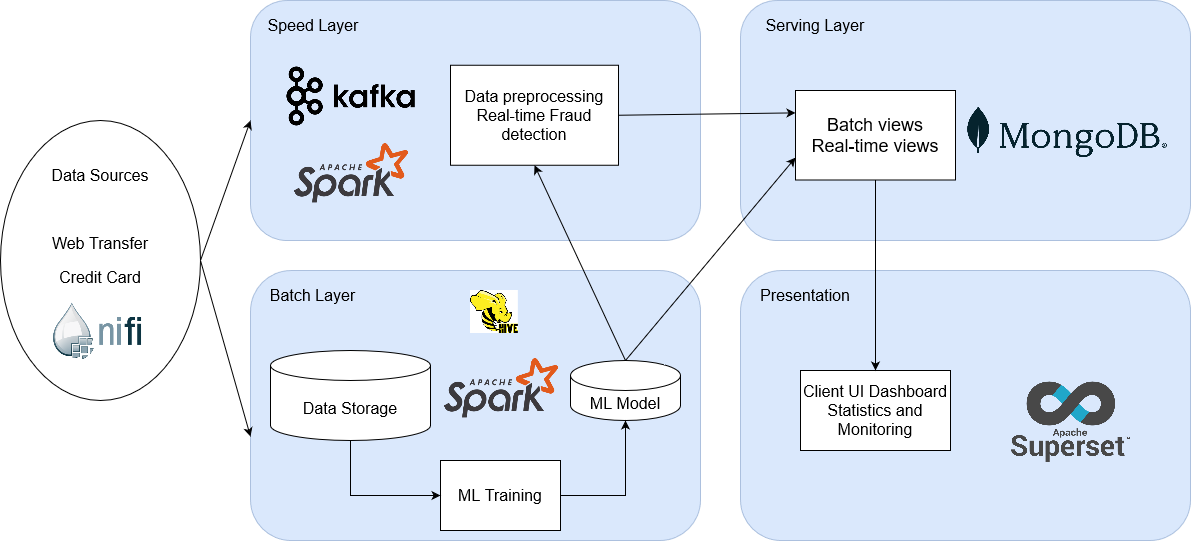
\includegraphics[width=0.95\textwidth]{images/Architecture-M2.png}
    \caption{Project architecture}
    \label{fig:sunset}
\end{figure}

The following Big Data platforms will be used:
\begin{itemize}
    \item Apache NiFi: to collect and distribute the data from different sources;
    \item Apache Hive as a data storage;
    \item Apache Kafka: to work with the streaming data;
    \item Apache Spark: to make the batch processing and model training;
    \item MongoDB: to store prepared batch view and real-time views for fast quering;
    \item Apache Superset (to be agreed with the supervisor): for data analysis on the user-interface. If the service will not be approved, UI will be implemented from scratch using JS framework, e.g. React.
\end{itemize}

\section{Planned ML tasks}

TBD

\section{Planned batch and stream processing}

TBD - The planned use of batch and stream processing for individual tasks

\section{Planned way of presenting the results}

TBD - Planned way of presenting the results to end-users in the further part of the project


\newpage

\section{Tasks assignment}

The table below contains the list of team members and preliminary allocation of tasks to team members.

\begin{table}[htbp]
\centering
\begin{tabular}{|p{4cm}|p{6cm}|p{4cm}|}
\hline
\textbf{Team member} & \textbf{Tasks} & \textbf{Supporter} \\
\hline
Salveen Singh Dutt & Batch processing of the historical data for up-to-date model training (Batch Layer). & Karina Tiurina \\
\hline
Karina Tiurina & Fraud detection model training and fine-tuning; Data stream processing (Speed Layer). & Salveen Singh Dutt \\
\hline
Mikołaj Malec & Data ingestion, collection and pre-processing. & Patryk Prusak  \\
\hline
Patryk Prusak & Data visualisation and configuration on the UI (Serving Layer). & Mikołaj Malec \\
\hline
\end{tabular}
\caption{Tasks assignment}
\end{table}


\end{document}